\documentclass{book}
\usepackage{ctex}
\usepackage{amsmath}
\usepackage{graphicx}
\usepackage{wrapfig}
\usepackage{caption}
\usepackage[top=0.8in, bottom=0.8in,left=0.8in, right=0.8in]{geometry}
\usepackage{float} 
\usepackage{subfigure}
\usepackage{subcaption}
\usepackage{bm}
\usepackage{setspace}
\xeCJKsetup{CJKmath=true} 
\title{量子力学讲义}
\author{David Tong\ 著\\胡锦浩\ 译}
\date{}
\begin{document}
\maketitle
\section*{推荐书目和资源}
目前在优秀的量子力学教材方面有短缺。下面是两本适合入门的书,与本课程程度差不多,它们是:
\begin{itemize}
    \item David. J. Griffiths, \textit{“Introduction to Quantum Mechanics”}
    \item Alasdair Rae, \textit{“Quantum Mechanics”}
\end{itemize}
\par
这两本书在给出清晰的概念和简单的解释,如果你在为你自己的基础挣扎的话可以参考。但是他们的讲法过于陈旧对后续的课程没有太多帮助
\par
如果你想要一本书可以毕生阅读的,而不仅仅是一年,那有很多教材可选,这里推荐我喜欢的
\begin{itemize}
    \item Shankar, \textit{“Principles of Quantum Mechanics”}
\end{itemize}
一本很长很详细的书,但是作者会带领你优雅的进行一些复杂计算
\begin{itemize}
    \item Landau and Lifshitz Volume 3, \textit{“Quantum Mechanics: Non-Relativistic Theory”}
\end{itemize}
朗道没有手把手教你最基本的理论,仅仅只有百科全书式的信息,没有惊人的解释,但是可读性很强。
\begin{itemize}
    \item Steven Weinberg, \textit{“Lectures on Quantum Mechanics”}
\end{itemize}
温伯格总是值得倾听的
\tableofcontents
\chapter{绪论}%Introduction
% 恕我直言,量子力学的发现是人类文明史上最伟大的成就。\par
% 量子力学完全与我们熟悉的经典的、熟悉的、常识性的对世界的认识。它比科幻小说家的梦想更令人费解和不安。然而,它无疑是对宇宙的正确描述,让我们了解了我们周围世界。\par
% 量子力学的成功之处,在于回答了一些古老而又非常基本的问题。比如为什么物质是稳定的?太阳为什么会发光,为什么是黄色的?为什么所有固体不是导体就是绝缘体?但是,量子力学也开辟了我们以前不知道的领域,比如说物质的新状态,即组成物质的粒子变得纠缠,以至于它们可以被用来执行看似不可能的任务,到波动的亚原子世界,再到对信息的意义,和人们可以用它来实现什么的新理解。\par
% 虽然量子力学给出了所有问题的正确答案,但它的代价是——答案总是统计性质的。量子世界几乎没有确定性。当然,经典世界中也很少有确定性,但我们总能努力消除它们。在经典物理学中,知识就是力量:你知道的越多,不确定性就越小。这是因为经典概率总是与我们的无知有关,任何看似随机的经典系统都是因为我们很难(但绝不是不可能)知道内部发生了什么。\par
% 量子世界并非如此。随机性是真的,不可预测是固有的。我们没有任何方法来降低系统的不确定性。举例来说,如果一个粒子出现在一个地方的概率是 $\frac{1}{2}$,而出现在其他地方的概率是 $\frac{1}{2}$,这很可能是因为粒子真的同时出现在这两个地方。任何消除量子确定性的尝试都只会转移不确定性。正如我们将要看到的,量子粒子是不稳定的物体,观察的行为本身就会改变,干扰它们所具有的许多其他微妙特性。\par
% 这门课的目的是了解量子世界和理解一些量子世界中的的奇特现象。需要弄清楚的是,这是我们步入未知的一步,这里我们在经典物理中的直觉将不再是在量子时间中一个很好的领导。幸运的事,我们有更好的领导/
毫不夸张地说,量子力学的发现是人类历史上最伟大的成就。\par
量子力学的世界观与我们所熟悉的经典力学的世界观截然不同。它比科幻小说家的梦更让人捉摸不透。但是,量子力学无疑是对我们世界正确的描述。\par
量子力学的成功之处在于回答了一些基础问题。如物质为什么是稳定的?太阳为什么闪耀,以及为什么是黄色的?为什么固体不是导体就是绝缘体?同时,量子力学也开辟一些我们从未接触的领域,比如,新物态,组成物质的粒子变得纠缠,使其完成了一些看似不可能完成的任务。从波动的亚原子世界,再到对信息全新理解,人们可以实现更多东西。\par
尽管量子力学给出了所有问题的正确答案,但是付出的代价是一切答案都是统计性质的。在量子的世界中几乎没有确定性。当然,在经典世界中也很少有确定性,但是我们总是可以找到方法来消除不确定性。在经典物理中,知识就是力量:你知道的越多,你就可以更好的消除不确定性。这是因为经典的可能性总是与我们的无知所关联的,任何看似随机的经典系统,我们很难知道其内部发生了什么,但是这绝不是不可能的。\par
但这与量子世界不同。随机的才是正常的,不可预测是固有的。我们没有任何方法减少系统的不确定性。举个例子,如果一个粒子出现在某个地方的概率是$\frac{1}{2}$,而出现在其他地方的概率是$\frac{1}{2}$,很可能粒子真同时出现在这两个地方。任何消除不确定性的尝试都只能转移不确定性,就像墙纸中的气泡。正如我们将要看到的,量子物体是不确定的,观测他们的的行为会导致其本身性质发生变化,干扰他们所具有的奇妙特性。\par
这门课的目的是尝试了解和理解量子世界中的一些奇特现象。需要清楚的是,这是我们步入未知世界的第一步,我们在经典物理中形成的直觉,可能不再是量子世界中的一个很好的向导。幸运的是,我们有了一个更好的向导,就是我们的无知,我们会用数学语言来描述量子世界。在接下去的几节课,以及以后的课程中,我们的学习方法是,接受这种数学描述,并利用它来建立一种新的直觉,了解宇宙是如何运作的。
\section{波函数}%The Wavefunction
% The difference between quantum and classical mechanics does not involve just a small tweak. Instead it is a root and branch overhaul of the entire framework.\par
量子力学与经典力学的不同不是一点两点。相反,它是对整个物理框架的彻底改革。\par
% This is manifest from the very beginning as we can see by comparing how we describe the state of a system in the two frameworks. The state is the information that tells us all we need to know about the system at a fixed time, with the idea that the laws of physics will then dictate how the state evolves at all later times. Throughout these lectures we will deal only with the dynamics of a single particle. For the present discussion, we’ll think about a particle moving in $\mathbf{R}^3$\par
这一点从一开始就很明显,我们可以通过比较在两种框架下描述系统状态的方式看出。状态可以告诉我们某时刻系统的所有信息,通过物理定律,我们可以算出接下去每一时刻的系统的状态。 在接下去的课程中,我们只处理单个粒子的运动。就现在的讨论,我们只考虑在$\mathbf{R}^3$空间中运动的粒子。\par
% In the classical world, the state of the particle is determined by its position x and its velocity $\mathbf{v}=\dot{\mathbf{x}}$. If you specify both bits of information at some time $t_0$ then you can use the equation of motion $\mathbf{F} = m\ddot{\mathbf{x}}$ to determine $\mathbf{x}(t)$ and $\mathbf{v}(t)$ for all time. Importantly, it’s not enough to just know only, say, the position of the particle at $t = t_0$. You need both $\mathbf{x}(t_0)$ and $\mathbf{v}(t_0)$. Mathematically, this is because the equation of motion is a second order differential equation and so you need to specify two integration constants to get a unique solution.\par
在经典物理中,粒子的状态只由它的位置$\mathbf{x}$和它的速度$\mathbf{v}=\dot{\mathbf{x}}$决定。如果你在某个时间$t_0$知道这两个信息,那么你可以使用运动方程$\mathbf{F} = m\ddot{\mathbf{x}}$来确定接下去所有时间的$\mathbf{x}(t)$和$\mathbf{v}(t)$。
% In the quantum world, the state of a particle is determined by its wavefunction. This is a complex valued function
在量子世界中质点的状态,只由它的波函数确定。这是一个复值函数
\[
    \psi(\mathbf{x},t)
\]
% As we will see, if you know the wavefunction at some time, say $t_0$, then you have all the information that you need to determine the state at all other times.\par
我们将会看见,如果你知道某时刻$t_0$的波函数,那么你就可以得到之后所有时间确定状态所需的所有信息.\par
% The description in terms of the wavefunction is not a small amendment to classical mechanics. We’ve replaced the three position coordinates $\mathbf{x}\in \mathbf{R}^3$ with an infinite amount of information, a functions worth of information. Moreover, we haven’t speci- fied anything about the particle’s velocity; that information must also be contained, in some manner, in the wavefunction $\psi(\mathbf{x},t)$.\par
用波函数描述系统与经典力学截然不同。我们已经将三个位置坐标$\mathbf{x}\in \mathbf{R}^3$用一个有着无限有用信息的函数替代。此外,我们还没有说明粒子的速度;这个信息必须以某种方式包含在$\psi(\mathbf{x},t)$中。\par
% The wavefunction has a very simple interpretation. Or, more precisely, the modsquare of the wavefunction has a very simple interpretation. It tells us the probability that we will find a particle at a given position. The probability density $P$ for a particle to sit at point $\mathbf{x}$ is
波函数有一种非常简单的解释,或者说波函数的模方有一个非常简单的解释。 他告诉我们粒子出现在某一个位置的概率。粒子出现在$\mathbf{x}$处的概率$P$是
\[
P(\mathbf{x},t) =|\psi(\mathbf{x},t)|^2
\]
% This is known as the Born rule, after Max Born who first understood that quantum mechanics is a theory of probability rather than certainty.\par
这被称作\textit{Born定则}, Max Born 第一次意识到量子理论是一个概率的理论,而不是确定的理论。\par
% From the probability density, you can compute actual probabilities by multiplying by a volume: the probability that the particle sits in some small volume $\mathrm{d}V$ centred around point $\mathbf{x}$ is $P(\mathbf{x},t)\mathrm{d}V$ .\par
从概率密度的角度来说,你可以将概率密度乘上体积来计算粒子出现在某个小体积$\mathrm{d}V$中心附近的概率,其概率为$P(\mathbf{x},t)\mathrm{d}V$。\par
% In all other realms of science, probability arises because of our ignorance. If you throw a classical dice, and know its initial state with complete precision, then there is no doubt about what will happen. Once the dice leaves your hand, the probability that you will roll a six is either 0 or 1. If you were really good at solving differential equations, you could just figure out the answer and impress your friends. But, in most circumstances we don’t have a good knowledge of the initial state of the dice and, besides, differential equations are hard. So we just give up, admit that we don’t know what will happen, and say that the probability of rolling a six is $\frac{1}{6}$. Crucially, however,the introduction of probability is entirely due to our lack of knowledge; it is not an inherent property of the dice.\par
在所有其他的科学领域中概率的产生,是由于我们的不了解。 如果你扔一个骰子,并且完全精确地知道它的初始状态,那接下去会发生什么就毫无疑义了。 你可以扔到六点的概率不是0就是1。 如果你非常善于解微分方程,你可以就算出答案来震惊你的朋友。 但在绝大多数情况下,我们对初值条件的了解,并不是非常精确,另外,解微分方程非常困难。 所以我们放弃了,承认我们不知道将会发生什么,然后承认扔到六点的概率为$\frac{1}{6}$。 从上面的例子可以看出概率的来源,是因为我们对初值条件的不了解,而不是骰子本身的属性。
% This is not the case in quantum mechanics. The state $\psi(\mathbf{x},t)$ contains all the information about a particle and the probabilistic interpretation is not because of any failing on our part, but instead due to an inherent randomness in the quantum world. This is, to put it mildly, something of a departure from the Newtonian way of thinking.\par
但这与量子力学中不同。状态$\psi(\mathbf{x},t)$包含了关于一个粒子的所有信息,并且概率的产生不是由于我们的问题,而是量子世界内在的随机性。这与牛顿式的思考方式不同。
% The novelty in the wavefunction description of the particle might suggest other interpretations of the function $\psi(\mathbf{x},t)$. You might, for example, wonder if perhaps we shouldn’t think of a particle at all, but rather some fluid-like object, spread out over space. Such objects are commonplace in physics and are known as $fields$. The electric and magnetic fields are familiar examples. But that’s not the right way to think about the wavefunction. This is because we never observe a fragmented particle, one that’s lost its particle form and starts spreading jell-o like throughout space. Any measuring device that will allow you to determine whether a particle is in some designated region of space will return the answer yes or no. It won’t tell you “well, the particle’s a little bit here but mostly somewhere over there to the left”. The wavefunction doesn’t describe some real fluid; it is more nebulous. It is a wave only of probability.
用波函数描述粒子的这一种全新的方式,可能会给波函数$\psi(\mathbf{x},t)$带来不同的解释。比如说,我们根本不应该考虑质点, 而是空间分布像流体一样的分布的物体。 在物理中称之为\textit{场}。 电场和磁场是我们熟悉的例子. 但这\textit{不}是我们理解过函数的方式。 就是因为我们从来没有观测到过一个弥散的粒子,一个失去了粒子形式,开始像果冻一样在太空中扩散的粒子。任何让你确定一个粒子是否在某个区域的观测,只会返回是或者否。 观测不会告诉你,“这个粒子部分在这里,但大部分在其他地方。”波函数不能描述真实的流体;它更加模糊,只能表示概率。
\begin{figure}[h]
    \centering
    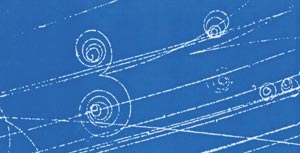
\includegraphics{img/1.jpg}
    % \caption{In any particular experiment, you only detect particles with very definite trajectories and no hint of the more nebulous underlying wavefunction.}
    \caption{在任何的实验中,只能检测到具有明确轨迹的粒子,而没有波函数的迹象}
    % \label{fig:mesh1}
\end{figure}\par
% This is illustrated in Figure 1 which shows the tracks left by electrons and positrons as they pass through a detector known as a bubble chamber. The fast travelling particles move in approximately straight lines, while those that are slower spiral in circles due to an applied magnetic field. The electrons bend one way, the positrons the other, giving the back-to-back spirals that you can see. For our purposes, the key point is that when the particles entered the detector, they were described by a wavefunction that was spread out over a large part of space. Yet, the particles don’t appear as fluffy, insubstantial clouds of probability. Instead, they leave clear tracks, with a definite trajectory.\par
图1显示了正电子和负电子穿过云室时的轨迹。 快速运动的粒子大约沿直线前进, 那些运动的比较慢的粒子,在磁场的作用下作螺旋运动。 电子向一个方向旋转,同时正电指向另一个方向旋转。 我们认为粒子进入探测器时,它们是由一个分布在很大空间中的波函数所描述的。 但是这些粒子并没有任何弥散的现象。 相反,他们有明确的轨迹。
% The introduction of probability at such a fundamental level means that we must abandon the idea of predicting, with certainty, what will happen in a given experiment. There is no way to say when and where the spirals will appear in the picture above. We can only compute the likelihood for this to happen. Clearly this is retrograde step from the Newtonian (strictly, Laplacian) dream of knowing everything that will happen, from the beginning to the end of time.\par
在如此基本的地方就引入概率,意味着我们必须要放弃精准预测的想法。 我们没有办法精准预测,在哪个地方会出现螺旋。 我们只能计算它的可能性。 显然这打破了Newton(准确来说,是Laplace)的梦想,即知道从开始到结束发生的一切。\par
% One might wonder if perhaps it’s possible to restore this dream at some deeper level. Maybe the wavefunction $\psi(\mathbf{x},t)$ is just some coarse-grained description of something finer and more subtle that’s going on underneath. Maybe another layer of reality awaits discovery, one that allows us to bring back our comfortable deterministic, Newtonian way of thinking. There is good reason to think that this is not the case. Reality is, at heart, probabilistic. We’ll mention some of the arguments for this in Section 3.5 where we touch upon some of the interpretations of quantum mechanics. A fuller description of why a deterministic world is incompatible with experiment will be given in the the lectures on Topics in Quantum Mechanics (see, in particular, the section on Quantum Foundations). For now, you’ll just have to accept that the world in which we live is not the one our forefathers grew up believing in. It is random and uncertain. It is also, as we will see, considerably more interesting because of it.
一些人可能会希望从更基本的地方来实现这一梦想。 可能波函数$\psi(\mathbf{x},t)$只是对接下去发生的更加精妙的事情的一个粗略的描述。 或者波函数有另一种解释,等待着我们去发现,让我们可以回到用更加舒适的Newton方法思考问题。 有充分的理由让我们不该这么做。 从本质上讲现实是概率的。 我们将在\S 3.5的时候遇到在这方面的讨论。 一个更加全面的描述为什么决定论的世界和实验是不相融的, 将会在量子力学专题研究\footnote{这是David Tong的另外一本讲义,可以在https://www.damtp.cam.ac.uk/user/tong/topicsinqm.html处找到——译者注}中描述(特别是在量子基本原理部分)。现在,你只能接受这一事实:我们生活的世界与我们的祖先从小所信仰的世界不同。它是随机和不确定的。我们将看到的,世界也因此变得有意思。


\subsection{归一化}%Normalisation
% The probabilistic interpretation means that the wavefunction can't just be any old function. The particle has to be somewhere, and this translates to the requirement
归一化后的函数将不与原来的波函数不同。它将转化为粒子在某位置的概率,这意味着
\[
\int \mathrm{d}^{3}xP(\mathbf{x},t)=\int\mathrm{d}^{3}x|\psi(\mathbf{x},t)|^{2}=1 
\]
% Wavefunctions that have this property are said to be \textit{normalised}.\par
波函数的这一性质称之为\textit{归一化}\par
% In practice, this isn't such a big deal. Suppose that we have a wavefunction $\psi(\mathbf{x},t)$ that isn't normalised but instead obeys
这没什么大不了的。假设我们有一个波函数$\psi(\mathbf{x},t)$,它不是归一化的,而是服从的
\[
\int \mathrm{d}^{3}x|\Psi({\mathbf{x}},t)|^{2}=N<\infty 
\]
% If $N$ is finite we say that the wavefunction is \textit{normalisable}. Clearly a wavefunction is normalisable only if $\psi[{\mathbf{x}},t] \to 0$ sufficiently fast as $|\mathbf{x}|\to\infty$ In this case,we can always construct a normalised wavefunction
如果$N$是有限的,那这个波函数就称之为\textit{可归一化的}. 显然一个波函数如果是可归一化的当且仅当在$|\mathbf{x}|\to\infty$时$\psi({\mathbf{x}},t) \to 0$。 在这种情况下,我们总是可以构造一个归一化的波函数。
\[
\psi(\mathbf{x},t)={\frac{1}{\sqrt{N}}}\Psi(\mathbf{x},t) 
\]
% Quite often in these lectures, it will turn out the be useful to work with un-normalised wavefunctions $\Psi$  and then remember to include the normalisation factor only at the end when computing probabilities.\par
在本课程中,我们经常会发现用未归一化的波函数 $\Psi$ 是很有用的,只要记住在计算概率的时候,再将它归一化即可。\par
% From the discussion above,it should be clear that we will have little use for wavefunctions that cannot be normalised because
从上面的讨论中,我们可以得到无法归一化的波函数,只有一点用,因为
\[
\int \mathrm{d}^{3}x|\psi({\mathbf{x}},t)|^{2}=\infty 
\]
% These have no probabilistic interpretation and should be discarded. They do not describe quantum states.(I should warn you that this statement, while mostly true, comes with small and annoying caveat that will rear its head fairly soon. We will address this in Section 2.1.)\par
这样的波函数没有概率解释。 他们也不表示任何量子态。(需要知道的是,这句话绝大多数情况下是正确的,但是我们将在\S 2.1中遇到反例).\par
% There is one other relation between wavefunctions that is important: two wavefunctions that differ by a constant, complex phase should actually be viewed as describing equivalent states.
波函数之间还有一个非常重要的关系,就是当两个波函数仅相差一个常数相位时,它们表示等价的状态.
\[
    \psi(\mathbf{x},t)\equiv e^{\mathbf{i}\alpha}\psi(\mathbf{x},t)
\]
% for any constant, real $\alpha$. Note, in particular, that this doesn’t change the probability distribution $P = |\psi|^2$. Nor, it will turn out, does it change anything else either. (The “anything else” argument is important here. As we’ll see later, if you multiplied the wavefunction by a spatially varying phase $e^{\mathbf{i}\alpha(\mathbf{x})}$ then it doesn’t change the probability distribution $P = |\psi|^2$ but it does change other observable quantities and so multiplying by such a factor does not give back the same state.)\par
 在多数情况下,实$\alpha$, 在一般情况下并不改变概率, 但是会改变一些别的东西(对“别的东西”的讨论在这里是很重要的。 我们将会看见,如果你给一个波函数乘上一个相位$e^{\mathbf{i}\alpha(\mathbf{x})}$  他并不会改变概率分布$P = |\psi|^2$ 但它会影响观测,所以并不会得到同一状态)\par
% Combining the need for normalisation, together with the phase ambiguity, it is sometimes useful think of states as the collection of normalisable, complex functions with the equivalence relation
结合归一化要求与对相位的不敏感性, 有时我们可以把态当作是一系列归一化的复函数的集合是十分有用的。
\[
    \psi(\mathbf{x},t)\equiv\lambda \psi(\mathbf{x},t)
\]
% for any complex $\lambda \in \mathbf{C}$ with $\lambda \ne 0$. The wavefunctions $\psi$ and $\lambda \psi$ should be viewed as describing the same physical state. 
对于任何复数$\lambda \in \mathbf{C}$且$\lambda \ne 0$。波函数$\psi$和$\lambda \psi$应被视为描述相同的态。
\subsection{叠加原理}%Superposition
% The set of wavefunctions form a vector space. This means that if $\psi_1(\mathbf{x},t)$ and $\psi_2(\mathbf{x},t)$ are both possible states of the system, then so too is
 波函数的结合构成一个矢量空间。 如果$\psi_1(\mathbf{x},t)$和$\psi_2(\mathbf{x},t)$都是系统的可能状态,那么系统状态也可能是
\[
    \psi_3(\mathbf{x},t)=\alpha\psi_1(\mathbf{x},t) +\beta\psi_2(\mathbf{x},t) 
\]
% for any $\alpha, \beta \in \mathbf{C}$. This is known as the \textit{principle of superposition}.\par
对于任意$\alpha, \beta \in \mathbf{C}$成立,这被称作\textit{叠加原理}.\par
% The mathematics underlying this statement is simple. If $\psi_1$ and $\psi_2$ are states of the system then both must be normalisable. They may, indeed, be normalised but for now let’s just assume that
这句话背后的数学原理非常简单。 如果$\psi_1$ 和$\psi_2$ 都是系统的状态,那它们必须是归一化的。 他们可能确实是归一化的,但我们现在在这里就假设
\[
    \int \mathrm{d}^3 x|\psi_i(\mathbf{x},t)|^2=N_i<\infty \ \ \mathrm{for}\ i=1,2
\]
% Then $\psi_3$ is also a possible state of the system provided that it too is normalisable. But it is straightforward to show that it has this property. First we have
那么$\psi_3$ 同样也是一个系统可能的状态,只要它是可归一化的。 这个性质很容易证明,首先有
\[
\int \mathrm{d}^3 x|\psi_3|^2=\int\mathrm{d}^3 x|\alpha\psi_1+\beta\psi_2|^2\le\int\mathrm{d}^3x \left(|\alpha\psi_1|+|\beta\psi_2|\right)^2
\]
% where we’ve used the triangle inequality $|z_1 + z_2| \le |z_1| + |z_2|$ for any $z_1, z_2 \in \mathbf{C}$. Continuing, we have
这里我们使用了三角不等式 $|z_1 + z_2| \le |z_1| + |z_2|$ 对于任意 $z_1, z_2 \in \mathbf{C}$. 继续, 我们有
\[
\int \mathrm{d}^3 x|\psi_3|^2\le\int \mathrm{d}^3 x\left(|\alpha\psi_1|^2+|\beta\psi_2|^2+2|\alpha\psi_1||\beta\psi_2| \right)\le\int \mathrm{d}^3 x\left(2|\alpha\psi_1|^2+2|\beta\psi_2|^2\right)
\]
% where, now, in the last step we’ve used the fact that $(|z_1|−|z_2|)^2 \ge 0$ which, rearranging, gives $2|z_1||z_2| \le |z_1|^2 + |z_2|^2$. So, finally, we get the result we wanted     
接下去,最后一步我们用了 $(|z_1|−|z_2|)^2 \ge 0$ 可以得到$2|z_1||z_2| \le |z_1|^2 + |z_2|^2$. 最后我们得到了我们想要的
\[
\int \mathrm{d}^3 x|\psi_3|^2\le 2|\alpha|^2N_1+2|\beta|^2 N_2<\infty
\]
% We learn that $\psi_3$ is normalisable, and hence also an allowed state of the system.\par
 现在我们知道$\psi_3$ 是可归一化的,所以这也是系统允许态。\par
% The idea that functions form a vector space might be novel. There is a simple notational trick that should help convince you that it’s not too far from things you’ve seen already. If we have some n-dimensional vector$\vec{y}$  then we often use subscript notation and write it as $y_i$ with $i = 1,\dots,N$ . We could equally well write it as $y(i)$ with $i = 1,\dots,N$ . A function $y(x)$ is a similar kind of object, but now with a continuous label $x \in \mathbf{R}$ rather than the discrete label $i = 1,\dots,N$.\par
波函数构成一个矢量空间的想法看上去非常新奇。 下面的一个技巧可以让你使这个东西看上去与你已知的东西相没那么远。 如果你有一个$n$维的矢量,我们将会将它写作我们约定的符号,如$y_i$ 其中 $i = 1,\dots,N$。 我们可以等价的将它写作$y(i)$ 其中 $i = 1,\dots,N$。函数 $y(x)$ 设类似的,只不过 $x \in \mathbf{R}$是连续的而不是像$i = 1,\dots,N$这样的离散指标.\par
% Of course, the big difference is that we’re now dealing with an infinite dimensional vector space rather than a finite dimensional vector space, and I would be lying if I told you that this doesn’t bring new issues to the table. Indeed, we’ve already met one of them above: we don’t consider any old function $\psi(\mathbf{x})$ to be in our vector space, but rather only normalisable functions. There are many further subtleties in store but we will be best served by simply ignoring them at this point. We’ll return to some issues in Section 3.\par
当然,现在我们处理的是无限维矢量空间,而不是有限维矢量空间, 但这并不会带来任何新的问题。 其实我们在上面已经遇见过了:在我们的矢量空间我们不考虑任何未归一化的函数$\psi(\mathbf{x})$而只考虑归一化的函数。 但其中还有很多微妙的地方在这里,我们暂时不处理。我们将在\S 3种讨论他们。\par
% The principle of superposition has profound physical consequences. Suppose that you have a particle that, at some time $t_0$, you know is localised somewhere near the point $\mathbf{X}$. For example, we could describe it by the Gaussian wavefunction.
叠加原理在物理中还有很多深远影响。 假如有一个粒子在$t_0$时刻,你知道他在 $\mathbf{X}$位置附近。 举个例子,你可以用高斯波函数来描述它。
\[
    \psi(\mathbf{x})=\dfrac{1}{\sqrt{N}}e^{-a(\mathbf{x}-\mathbf{X})^2}
\]
% for some choice of a that tells you how spread out the wavefunction is. Here $N$ is a normalisation factor that won’t concern us. (For what it’s worth, we should take $N = (\pi/2a)^{3/2}$ if we want to ensure that $\psi$ is normalised.) This is a state in which you might imagine that the particle still retains something of its classical particle nature, at least in the sense that the probability distribution is not spread out over long distances. However, the superposition principle tells us that we should also entertain the idea that the particle can sit in a state
对于$a$的选择可以告诉你这个波的扩散程度。这里 $N$ 是一个归一化常数我们无需考虑它(其中$N = (\pi/2a)^{3/2}$,如果你想确定其是归一化的)在这种状态下,你可以想象粒子仍然保留了一些经典粒子的性质,至少概率分布没有在长距离上分散。然而,叠加原理告诉我们,我们还应该考虑粒子可以处于某种状态的想法
\[
    \psi(\mathbf{x})=\dfrac{1}{\sqrt{N'}}(e^{-a(\mathbf{x}-\mathbf{X_1})^2}+e^{-a(\mathbf{x}-\mathbf{X_2})^2})
\]
% for arbitrary positions $\mathbf{X_1}$ and $\mathbf{X_2}$. But now the cat is really out of the bag! The interpretation of this state is that the particle has somehow split and now sits both near $\mathbf{X_1}$ and near $\mathbf{X_2}$. Indeed, we’ll shortly see clear experimental consequences of states like the one above, where elementary particles – which are, as far as we can tell, indivisible – are coaxed into travelling along two or more different paths simultaneously. Taken to the logical extreme, it is states like the one above that lead us to seemingly paradoxical situations with cats that are both alive and dead.
对于任意位置$\mathbf{X_1}$和$\mathbf{X_2}$。但是现在可以清楚了!对这种状态的解释是,粒子以某种方式分裂了,可以位于$\mathbf{X_1}$和$\mathbf{X_2}$附近。事实上,我们很快就会看到上述状态的清晰实验结果。据我们所知,经典粒子它们是不可分割的——它同时沿着两条或更多不同的路径运动。从极端情况考虑,正是像上面这样的状态导致了薛定谔猫的情况的出现。


\section{薛定谔方程}%The Schr$\ddot{o}$dinger Equation
\subsection{哈密顿算符}%The Hamiltonian
\subsection{概率守恒}%Conservation of Probability
\subsection{波函数的坍缩}%The Collapse of the Wavefunction
\section{双缝实验}%The Double Slit Experiment
\chapter{一维中量子问题}%A Quantum Particle in One Dimension
\section{自由粒子}%The Free Particle
\subsection{圆上粒子}%A Particle on a Circle
\subsection{无限深势阱}%The Infinite Potential Well
\subsection{高斯包波}%The Gaussian Wavepacket
\subsection{初见期望值}%A First Look at Expectation Values
\section{谐振子}%The Harmonic Oscillator
\subsection{能谱}%The Energy Spectrum
\subsection{波函数}%The Wavefunctions
\section{束缚态}%Bound States
\subsection{有限深势阱}%A Finite Potential Well
\subsection{$\delta$函数势}%A Delta Function Potential
\subsection{一些更广泛的结论}%Some General Results
\subsection{双势阱}%The Double Well Potential
\section{散射}%Scattering
\subsection{阶梯势}%A Step Potential
\subsection{隧穿效应}%Tunnelling
\chapter{量子力学的表示}%The Formalism of Quantum Mechanics
\section{态}%States
\subsection{内积}%The Inner Product
\section{算符与可观测量}%Operators and Observables
\subsection{本征函数与本征值}%Eigenfunctions and Eigenvalues
\subsection{厄米算符}%Hermitian Operators
\subsection{动量本征值与傅立叶变换}%Properties of Hermitian Matrices
\section{Measurement}%
\subsection{期望值}%Measurement
\section{Commutation Relations}%
\subsection{The Heisenberg Uncertainty Principle}
\section{Interpretations of Quantum Mechanics}
\subsection{Hidden Variables}
\subsection{Copenhagen and Many Worlds}
\subsection{Shut Up and Calculate}
\chapter{A Quantum Particle in Three Dimensions}
\section{Angular Momentum}
\subsection{Angular Momentum Commutation Relations }
\subsection{The Eigenfunctions are Spherical Harmonics}
\section{Solving the 3d Schr ̈odinger Equation}
\subsection{The 3d Harmonic Oscillator}
\subsection{Bound States in 3d}
\subsection{Why Can’t the Wavefunction Diverge at the Origin?}
\section{The Hydrogen Atom}
\subsection{The Energy Spectrum}
\subsection{The Wavefunctions}
\section{A Pre-Quantum Quantum History}
\subsection{The Bohr Model}
\subsection{What About the Photon?}
\section{A First Look at Renormalisation}
\subsection{A Delta Function Potential in the Plane}
\subsection{Renormalisation in Quantum Mechanics}

\end{document}